\section{Temat i cel projektu}
\label{sec:temat}

\subsection{Opis problemu}
\label{sec:problem}

Dron zwiadowczy startuje z bazy umieszczonej na dwuwymiarowej mapie
podzielonej na pola. Jego zadaniem jest wykonanie zdjęć $K$ celów
rozmieszczonych na mapie i powrót do bazy. Misję utrudniają:

\begin{itemize}
  \item \textbf{ograniczona bateria} -- każdy krok zużywa energię, a jej
        uzupełnienie jest możliwe wyłącznie na stacjach ładowania, które nie
        leżą na najkrótszych trasach między celami;
  \item \textbf{przeszkody statyczne} -- budynki, przez które nie można przelecieć;
  \item \textbf{strefy radarowe} -- przebywanie w nich skraca trasę, ale w
        każdym kroku grozi wykryciem drona i niepowodzeniem misji;
  \item \textbf{patrol} -- przeszkoda dynamiczna poruszająca się cyklicznie
        po stałej trasie; kontakt z patrolem kończy misję;
  \item \textbf{zdarzenie zależne od decyzji agenta} -- sfotografowanie
        celu nr~1 powoduje zamknięcie wybranego korytarza (pole $Z$), co może
        odciąć krótszą drogę do pozostałych celów.
\end{itemize}

Agent nie zna z góry modelu środowiska (prawdopodobieństwa wykrycia, skutków
zdarzeń) -- uczy się wyłącznie na podstawie interakcji. Projekt zakłada kilka
map o rosnącej trudności (\emph{easy}, \emph{medium}, \emph{hard}).
Przykładową mapę pokazano na rys.~\ref{fig:map-easy}.

\begin{figure}[h]
  \centering
  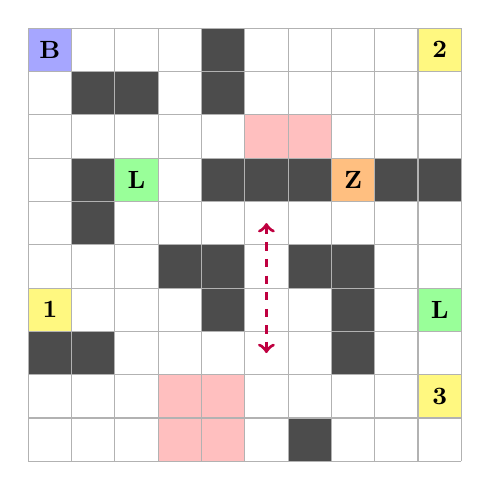
\begin{tikzpicture}[scale=0.55]
  \fill[blue!35] (0,9) rectangle ++(1,1);
  \node at (0.5,9.5) {\small\textbf{B}};
  \fill[white] (1,9) rectangle ++(1,1);
  \fill[white] (2,9) rectangle ++(1,1);
  \fill[white] (3,9) rectangle ++(1,1);
  \fill[black!70] (4,9) rectangle ++(1,1);
  \fill[white] (5,9) rectangle ++(1,1);
  \fill[white] (6,9) rectangle ++(1,1);
  \fill[white] (7,9) rectangle ++(1,1);
  \fill[white] (8,9) rectangle ++(1,1);
  \fill[yellow!50] (9,9) rectangle ++(1,1);
  \node at (9.5,9.5) {\small\textbf{2}};
  \fill[white] (0,8) rectangle ++(1,1);
  \fill[black!70] (1,8) rectangle ++(1,1);
  \fill[black!70] (2,8) rectangle ++(1,1);
  \fill[white] (3,8) rectangle ++(1,1);
  \fill[black!70] (4,8) rectangle ++(1,1);
  \fill[white] (5,8) rectangle ++(1,1);
  \fill[white] (6,8) rectangle ++(1,1);
  \fill[white] (7,8) rectangle ++(1,1);
  \fill[white] (8,8) rectangle ++(1,1);
  \fill[white] (9,8) rectangle ++(1,1);
  \fill[white] (0,7) rectangle ++(1,1);
  \fill[white] (1,7) rectangle ++(1,1);
  \fill[white] (2,7) rectangle ++(1,1);
  \fill[white] (3,7) rectangle ++(1,1);
  \fill[white] (4,7) rectangle ++(1,1);
  \fill[red!25] (5,7) rectangle ++(1,1);
  \fill[red!25] (6,7) rectangle ++(1,1);
  \fill[white] (7,7) rectangle ++(1,1);
  \fill[white] (8,7) rectangle ++(1,1);
  \fill[white] (9,7) rectangle ++(1,1);
  \fill[white] (0,6) rectangle ++(1,1);
  \fill[black!70] (1,6) rectangle ++(1,1);
  \fill[green!40] (2,6) rectangle ++(1,1);
  \node at (2.5,6.5) {\small\textbf{L}};
  \fill[white] (3,6) rectangle ++(1,1);
  \fill[black!70] (4,6) rectangle ++(1,1);
  \fill[black!70] (5,6) rectangle ++(1,1);
  \fill[black!70] (6,6) rectangle ++(1,1);
  \fill[orange!50] (7,6) rectangle ++(1,1);
  \node at (7.5,6.5) {\small\textbf{Z}};
  \fill[black!70] (8,6) rectangle ++(1,1);
  \fill[black!70] (9,6) rectangle ++(1,1);
  \fill[white] (0,5) rectangle ++(1,1);
  \fill[black!70] (1,5) rectangle ++(1,1);
  \fill[white] (2,5) rectangle ++(1,1);
  \fill[white] (3,5) rectangle ++(1,1);
  \fill[white] (4,5) rectangle ++(1,1);
  \fill[white] (5,5) rectangle ++(1,1);
  \fill[white] (6,5) rectangle ++(1,1);
  \fill[white] (7,5) rectangle ++(1,1);
  \fill[white] (8,5) rectangle ++(1,1);
  \fill[white] (9,5) rectangle ++(1,1);
  \fill[white] (0,4) rectangle ++(1,1);
  \fill[white] (1,4) rectangle ++(1,1);
  \fill[white] (2,4) rectangle ++(1,1);
  \fill[black!70] (3,4) rectangle ++(1,1);
  \fill[black!70] (4,4) rectangle ++(1,1);
  \fill[white] (5,4) rectangle ++(1,1);
  \fill[black!70] (6,4) rectangle ++(1,1);
  \fill[black!70] (7,4) rectangle ++(1,1);
  \fill[white] (8,4) rectangle ++(1,1);
  \fill[white] (9,4) rectangle ++(1,1);
  \fill[yellow!50] (0,3) rectangle ++(1,1);
  \node at (0.5,3.5) {\small\textbf{1}};
  \fill[white] (1,3) rectangle ++(1,1);
  \fill[white] (2,3) rectangle ++(1,1);
  \fill[white] (3,3) rectangle ++(1,1);
  \fill[black!70] (4,3) rectangle ++(1,1);
  \fill[white] (5,3) rectangle ++(1,1);
  \fill[white] (6,3) rectangle ++(1,1);
  \fill[black!70] (7,3) rectangle ++(1,1);
  \fill[white] (8,3) rectangle ++(1,1);
  \fill[green!40] (9,3) rectangle ++(1,1);
  \node at (9.5,3.5) {\small\textbf{L}};
  \fill[black!70] (0,2) rectangle ++(1,1);
  \fill[black!70] (1,2) rectangle ++(1,1);
  \fill[white] (2,2) rectangle ++(1,1);
  \fill[white] (3,2) rectangle ++(1,1);
  \fill[white] (4,2) rectangle ++(1,1);
  \fill[white] (5,2) rectangle ++(1,1);
  \fill[white] (6,2) rectangle ++(1,1);
  \fill[black!70] (7,2) rectangle ++(1,1);
  \fill[white] (8,2) rectangle ++(1,1);
  \fill[white] (9,2) rectangle ++(1,1);
  \fill[white] (0,1) rectangle ++(1,1);
  \fill[white] (1,1) rectangle ++(1,1);
  \fill[white] (2,1) rectangle ++(1,1);
  \fill[red!25] (3,1) rectangle ++(1,1);
  \fill[red!25] (4,1) rectangle ++(1,1);
  \fill[white] (5,1) rectangle ++(1,1);
  \fill[white] (6,1) rectangle ++(1,1);
  \fill[white] (7,1) rectangle ++(1,1);
  \fill[white] (8,1) rectangle ++(1,1);
  \fill[yellow!50] (9,1) rectangle ++(1,1);
  \node at (9.5,1.5) {\small\textbf{3}};
  \fill[white] (0,0) rectangle ++(1,1);
  \fill[white] (1,0) rectangle ++(1,1);
  \fill[white] (2,0) rectangle ++(1,1);
  \fill[red!25] (3,0) rectangle ++(1,1);
  \fill[red!25] (4,0) rectangle ++(1,1);
  \fill[white] (5,0) rectangle ++(1,1);
  \fill[black!70] (6,0) rectangle ++(1,1);
  \fill[white] (7,0) rectangle ++(1,1);
  \fill[white] (8,0) rectangle ++(1,1);
  \fill[white] (9,0) rectangle ++(1,1);
  \draw[step=1,gray!60] (0,0) grid (10,10);
  \draw[very thick,purple,dashed,<->] (5.5,5.5) -- (5.5,4.5) -- (5.5,3.5) -- (5.5,2.5);
\end{tikzpicture}

  \caption{Robocza mapa \emph{easy} ($10\times10$). B -- baza, 1--3 -- cele,
    L -- stacje ładowania, czerwone pola -- strefy radarowe, Z -- korytarz
    zamykany po sfotografowaniu celu~1, czarne pola -- przeszkody, fioletowa
    linia -- trasa patrolu (ruch tam i z powrotem).}
  \label{fig:map-easy}
\end{figure}

\paragraph{Dylemat zaprojektowany na mapie \emph{easy}.} Cel~1 leży najbliżej
bazy (6~kroków), ale jego sfotografowanie zamyka korytarz $Z$. Po tym
zdarzeniu jedyna droga do celu~2 prowadzi przez strefę radarową. Bezpieczna
kolejność to 2~$\rightarrow$~3~$\rightarrow$~1~$\rightarrow$~baza
(ok.\ 46 kroków po trasach omijających radary), co przekracza pojemność
baterii $E_{\max}=30$ -- agent musi więc dodatkowo zaplanować ładowanie.
Strategia zachłanna („najpierw najbliższy cel'') prowadzi natomiast do
konieczności lotu przez radar. Wartości zmierzono algorytmem BFS na mapie
z rys.~\ref{fig:map-easy}, bez uwzględnienia patrolu.

\subsection{Cel agenta}
\label{sec:cel}

Agent ma wykonać zdjęcia wszystkich celów i wrócić do bazy w możliwie małej
liczbie kroków, nie dopuszczając do wykrycia, kolizji z patrolem ani do
rozładowania baterii. Działanie agenta uznajemy za poprawne, jeżeli epizod
kończy się sukcesem w rozumieniu sekcji~\ref{sec:koniec}, a za skuteczne --
jeżeli w fazie ewaluacji (bez eksploracji) agent osiąga sukces w większości
epizodów przy długości trasy zbliżonej do najkrótszej bezpiecznej trasy
z ładowaniem. Szczegółowe miary podano w sekcji~\ref{sec:miary}.
